While prior work has studied how to improve inference and tangentially explored the asymmetry between the encoder and decoder, we study that explicitly and across model scales. We focus our studies on \textbf{structural pruning} as inference gains are easy to realize, and this approach is highly compatible with other methods like quantization and unstructured pruning.\\
Following Shleifer et al., we adopt the \textbf{S}hink and \textbf{t}hen \textbf{f}ine (STF) tune approach for compression. First, a model is trained until convergence on a fine-tuning summarization task. Then, entire layers are removed from the encoder, decoder, or both, and the model is further fine-tuned until it has re-converged. \\
Each model we study has a uniform number of encoder and decoder layers, so we prune only the encoders, decoders, and a symmetric combination of the two combinations. We used our three scales of uncompressed models (small, base, large), and we pruned the model in multiples of 1 on the encoder, the decoder, and both. After pruning, models are fine-tuned again and evaluated. This means that for each dataset, we have 16 variants for each model size leading to 48 models per dataset and 144 models overall. \\
Given the wide number of models and the cost of multiple seeds or model-specific optimization, we train each model once and do not optimize the parameters for each model. While this leads to a worse-than-ideal performance, our goal is not to hyper-optimize models but explore where there is high sensitivity. To save space, we use the shorthand $l_{enc}$ and $l_{dec}$ to refer to the number portion of transformer encoder and decoder layers (out of 6), and $R$ refers to the percentage performance recall vs. uncompressed baseline. Detailed results have been moved to the \ref{appendix:asym-full} to save space.\\
\begin{table}[!ht]
    \centering
    \tiny
    \caption{Relation between scale and asymmetry on model performance on the CNNDM dataset}
    \scalebox{0.9}{
    \begin{tabular}{|l|l|l|l|l|l|l|l|}
    \hline
        \multicolumn{2}{l}{} &  \multicolumn{2}{l}{Small} & \multicolumn{2}{l}{Base} & \multicolumn{2}{l}{Large}  \\ \hline 
        $l_{enc}$ & $l_{dec}$ & R-2 & $R$ & R-2 & $R$ & R-2 & $R$ \\ \hline
        6 & 6 & 17.55 & 100.00\% & 19.77 & 100.00\% & 21.15 & 100.00\% \\ \hline
        6 & 5 & 17.68 & 100.74\% & 19.92 & 100.76\% & 21.30 & 100.69\% \\ \hline
        6 & 4 & 17.27 & 98.36\% & 19.85 & 100.42\% & 21.32 & 100.81\% \\ \hline
        6 & 3 & 16.40 & 93.43\% & 18.85 & 95.37\% & 21.08 & 99.66\% \\ \hline
        6 & 2 & 15.35 & 87.42\% & 18.68 & 94.51\% & 20.67 & 97.73\% \\ \hline
        6 & 1 & 11.33 & 64.57\% & 16.48 & 83.38\% & 19.49 & 92.12\% \\ \hline
        \midrule
        5 & 6 & 17.69 & 100.81\% & 19.92 & 100.76\% & 21.13 & 99.88\% \\ \hline
        4 & 6 & 17.35 & 98.84\% & 19.67 & 99.50\% & 20.83 & 98.47\% \\ \hline
        3 & 6 & 16.80 & 95.70\% & 18.85 & 95.37\% & 20.53 & 97.06\% \\ \hline
        2 & 6 & 15.54 & 88.51\% & 18.22 & 92.14\% & 19.74 & 93.33\% \\ \hline
        1 & 6 & 13.31 & 75.83\% & 17.06 & 86.27\% & 18.68 & 88.31\% \\ \hline
        \midrule
        5 & 5 & 17.07 & 97.23\% & 19.72 & 99.74\% & 21.23 & 100.34\% \\ \hline
        4 & 4 & 16.20 & 92.28\% & 19.17 & 96.99\% & 20.90 & 98.81\% \\ \hline
        3 & 3 & 14.91 & 84.95\% & 17.46 & 88.29\% & 20.13 & 95.16\% \\ \hline
        2 & 2 & 11.97 & 68.17\% & 15.87 & 80.26\% & 18.47 & 87.30\% \\ \hline
        1 & 1 & 6.05 & 34.45\% & 12.23 & 61.88\% & 15.51 & 73.32\% \\ \hline
    \end{tabular}}
    \label{tab:cnndm-r2-asym}
\end{table}
\begin{table}[!ht]
    \centering
    \tiny
    \caption{Scale and Pruning on XSUM dataset}
    \scalebox{0.9}{
    \begin{tabular}{|l|l|l|l|l|l|l|l|}
    \hline
        \multicolumn{2}{l}{} &  \multicolumn{2}{l}{Small} & \multicolumn{2}{l}{Base} & \multicolumn{2}{l}{Large}  \\ \hline 
        $l_{enc}$ & $l_{dec}$ & R-2 & $R$ & R-2 & $R$ & R-2 & $R$ \\ \hline
        6 & 6 & 11.09 & 100.00\% & 15.69 & 100.00\% & 16.34 & 100.00\% \\ \hline
        6 & 5 & 11.61 & 104.74\% & 15.27 & 97.35\% & 19.80 & 121.16\% \\ \hline
        6 & 4 & 11.43 & 103.12\% & 14.91 & 95.03\% & 19.30 & 118.09\% \\ \hline
        6 & 3 & 11.24 & 101.36\% & 15.40 & 98.17\% & 18.92 & 115.77\% \\ \hline
        6 & 2 & 10.53 & 94.98\% & 15.19 & 96.82\% & 17.96 & 109.93\% \\ \hline
        6 & 1 & 6.03 & 54.42\% & 13.73 & 87.53\% & 16.47 & 100.76\% \\ \hline
        \midrule
        5 & 6 & 11.18 & 100.82\% & 15.92 & 101.47\% & 19.43 & 118.88\% \\ \hline
        4 & 6 & 10.61 & 95.68\% & 14.10 & 89.91\% & 18.33 & 112.16\% \\ \hline
        3 & 6 & 10.11 & 91.16\% & 13.84 & 88.21\% & 16.90 & 103.39\% \\ \hline
        2 & 6 & 8.59 & 77.52\% & 12.10 & 77.12\% & 14.97 & 91.61\% \\ \hline
        1 & 6 & 7.70 & 69.43\% & 10.27 & 65.47\% & 12.52 & 76.63\% \\ \hline
        \midrule
        5 & 5 & 10.73 & 96.76\% & 15.72 & 100.22\% & 19.18 & 117.38\% \\ \hline
        4 & 4 & 10.19 & 91.96\% & 14.30 & 91.15\% & 17.56 & 107.43\% \\ \hline
        3 & 3 & 9.50 & 85.69\% & 12.44 & 79.32\% & 15.89 & 97.21\% \\ \hline
        2 & 2 & 7.31 & 65.91\% & 10.67 & 68.05\% & 12.15 & 74.34\% \\ \hline
        1 & 1 & 4.00 & 36.09\% & 7.74 & 49.35\% & 8.96 & 54.86\% \\ \hline
    \end{tabular}}
    \label{tab:xsum-r2-asym}
\end{table}
\subsection{Scale and Pruning}
Looking at abridged results in \ref{tab:qiws-r2-asym}, \ref{tab:cnndm-r2-asym}, and \ref{tab:xsum-r2-asym}, there is a clear scaling law as smaller models see much larger drops in performance when compressed to the same degree. For example, on the QIWS dataset, compression to $\frac{1}{6}$ of the layers on the encoder and decoder cause an 80\% drop in R-2 on a small model but only 40\% on the larger model. This scale comparison is 65\% to 26\% on CNNDM and 64\% to 45\% on XSUM datasets.\\
\begin{figure}
    \centering
    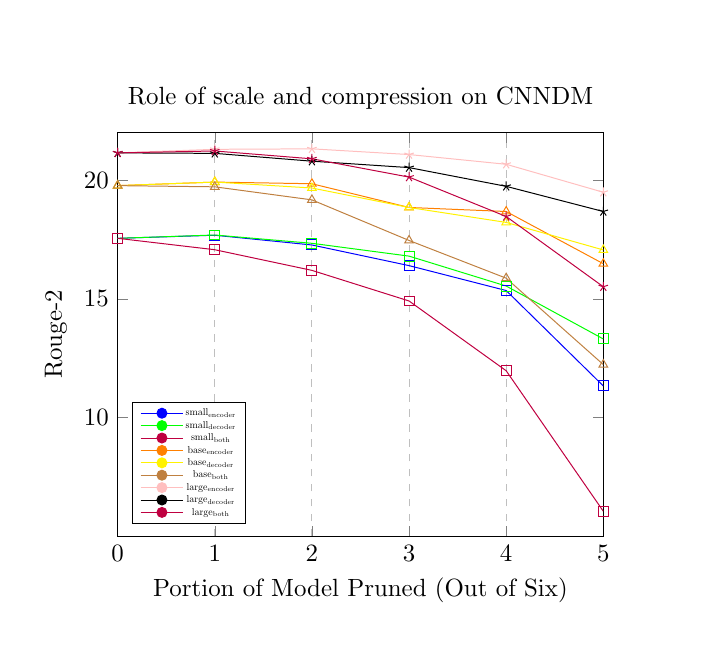
\begin{tikzpicture}
\scalebox{0.9}{
\begin{axis}[
    title={Role of scale and compression on CNNDM},
    ylabel={Rouge-2},
    xlabel={Portion of Model Pruned (Out of Six)},
    ymin=5, ymax=22,
    xmin=0, xmax=5,
    ytick={10,15,20},
    xtick={0,1,2,3,4,5},
    legend pos=south west,
    xmajorgrids=true,
    grid style=dashed,
    legend style={nodes={scale=0.4, transform shape}}, 
    legend image post style={mark=*}
]
\addplot[
    color=blue,
    mark=square,
    ]
    coordinates {
    (0, 17.55) (1, 17.68) (2, 17.27) (3, 16.4) (4, 15.35) (5,11.33)
    };
\addplot[
    color=green,
    mark=square,
    ]
    coordinates {
    (0, 17.55) (1, 17.69) (2, 17.34) (3, 16.8) (4,15.54 ) (5,13.31)
    };  
\addplot[
    color=purple,
    mark=square,
    ]
    coordinates {
    (0, 17.55) (1, 17.07) (2, 16.2) (3, 14.91) (4, 11.97) (5,6.05)
    };
\addplot[
    color=orange,
    mark=triangle,
    ]
    coordinates {
    (0, 19.77) (1, 19.92) (2, 19.85) (3, 18.85) (4, 18.68) (5,16.48)
    };
\addplot[
    color=yellow,
    mark=triangle,
    ]
    coordinates {
    (0, 19.77) (1, 19.92) (2, 19.67) (3, 18.85) (4,18.22 ) (5,17.06)
    };  
\addplot[
    color=brown,
    mark=triangle,
    ]
    coordinates {
    (0, 19.77) (1, 19.72) (2, 19.17) (3, 17.46) (4, 15.87) (5,12.23)
    };
\addplot[
    color=pink,
    mark=star,
    ]
    coordinates {
    (0, 21.15) (1, 21.30) (2, 21.32) (3, 21.08) (4, 20.67) (5,19.49)
    };
\addplot[
    color=black,
    mark=star,
    ]
    coordinates {
    (0, 21.15) (1, 21.13) (2,20.8 ) (3, 20.53) (4,19.74 ) (5,18.68)
    };  
\addplot[
    color=purple,
    mark=star,
    ]
    coordinates {
    (0, 21.15) (1, 21.23) (2, 20.9) (3, 20.13) (4, 18.47) (5,15.51)
    };
\legend{small\textsubscript{encoder}, small\textsubscript{decoder}, small\textsubscript{both}, base\textsubscript{encoder}, base\textsubscript{decoder}, base\textsubscript{both},large\textsubscript{encoder}, large\textsubscript{decoder}, large\textsubscript{both} }
 \end{axis}}
\end{tikzpicture}
    \caption{Relationship between model compression, model size, and summarization accuracy measured by rouge-2 vs. Number Layers. small\textsubscript{encoder} refers to a FLAN-T5 small which has only pruned the encoder, small\textsubscript{decoder} for only the decoder, and small\textsubscript{both} for the encoder and decoder}
    \label{fig:scale-laws-pruning}
\end{figure}
Similar scaling results hold with encoder or decoder pruning, where compressing large models lead to a 5x lower loss in performance than small models. As the model's size grows, the impact of decoder vs. encoder-only pruning becomes more muted. On the CNNDM dataset, the gap between the decoder only and encoder only pruned to $\frac{1}{6}$ is 10\% with the FLAN-T5 small but only 4\% with the large variant. When comparing asymmetric and symmetric, the gap is even further pronounced where the small gap is 30\% while the large is 20\%. \\
As shown in figure \ref{fig:scale-laws-pruning}, the impact of compression becomes more muted as the model size grows. In other words, larger models are more compressible and amenable to asymmetry in this compression. \\
The impact of asymmetry is easiest to understand as it is not surprising that complete pruning of a model leads to higher losses than partial pruning across datasets and model sizes. While this finding is not immediately surprising, evaluating the inference costs becomes important. \\
\subsection{Inference Benchmarks}
We evaluate the impact of asymmetry in a similar method to our scale experiments. Using an A10 GPU, we evaluate performance for summarization on a portion of each model's respective evaluation datasets with a max sequence length of 1024, a max summary length of 256, and batch sizes 1, 8, and 16. \\
\begin{table}[!htb!]
    \centering
    \tiny
    \scalebox{0.8}{
    \begin{tabular}{|l|l|l|l|l|l|l|l|}
    \hline
        \multicolumn{2}{l}{} &  \multicolumn{2}{l}{QIWS} & \multicolumn{2}{l}{CNN/DailyMail} & \multicolumn{2}{l}{XSUM}  \\ \hline 
        \midrule
        $l_{enc}$ & $l_{dec}$ & Impact & Speedup & Impact & Speedup & Impact & Speedup \\ \hline
        6 & 3 & -4.36\% & 1.80 & -0.34\% & 1.65 & 15.77\% & 1.64 \\ \hline
        6 & 2 & -5.99\% & 2.44 & -2.27\% & 2.03 & 9.93\% & 2.07 \\ \hline
        6 & 1 & -9.85\% & 3.83 & -7.88\% & 2.70 & 0.76\% & 2.71 \\ \hline
        3 & 6 & -8.42\% & 1.04 & -2.94\% & 1.14 & 3.39\% & 1.16 \\ \hline
        2 & 6 & -10.57\% & 1.04 & -6.67\% & 1.19 & -8.39\% & 1.21 \\ \hline
        1 & 6 & -18.89\% & 1.06 & -11.69\% & 1.27 & -23.37\% & 1.30 \\ \hline
        3 & 3 & -11.69\% & 1.91 & -4.84\% & 1.94 & -2.79\% & 2.06 \\ \hline
        2 & 2 & -17.62\% & 2.20 & -12.70\% & 2.78 & -25.66\% & 2.83 \\ \hline
        1 & 1 & -39.06\% & 2.44 & -26.68\% & 4.96 & -45.14\% & 4.84 \\ \hline
    \end{tabular}}
    \caption{Relationship between accuracy and speedup of encoder only, the decoder only, encoder and decoder pruning on FLAN-T5 Large models on CNN/DM, XSUM, and QIWS. Speedup is measured by comparing the improvements in latency for batch size one vs. the uncompressed baseline. The impact is the relative loss of Rouge-2 of compressed models vs. the uncompressed baseline.}
    \label{tab:asymetry-vs-speedup}
\end{table}\\
Looking at the focused set of results for large models across datasets in table \ref{tab:asymetry-vs-speedup} on the impact of R-2 vs. inference speedup, we can see a clear relationship between asymmetry and inference efficiency. While detailed inference results can be found in the appendix \ref{sec:inference-benchmarks} on this focused set of results, we can see that pruning only the encoder leads to no more than 30\% improvement in inference efficiency at a sizable loss in accuracy. Pruning the model symmetrically leads to realizable inference improvements of up to ~5x at the expense of summarization accuracy. \\ 
Alternatively, when only the decoder is pruned, it is possible to see most of the inference speedups seen during constant pruning with a substantially lower impact on accuracy. On the CNN/DM dataset, constant pruning leads to 8\% better inference but losses nearly four times the performance of non-uniform compression.  \\
\begin{table}[!htb!]
    \centering
    \small
    \scalebox{0.7}{
    \begin{tabular}{|l|l|l|l|l|l|l|l|}
    \hline
        \multicolumn{2}{l}{} &  \multicolumn{2}{l}{Small} & \multicolumn{2}{l}{Base} & \multicolumn{2}{l}{Large}  \\ \hline 
        \midrule
        $l_{enc}$ & $l_{dec}$ & Impact & Speedup & Impact & Speedup & Impact & Speedup \\ \hline
        6 & 6 & -3.76\% & 1.79 & -1.42\% & 1.76 & -4.36\% & 1.80 \\ \hline
        6 & 6 & -14.39\% & 2.69 & -6.62\% & 2.13 & -5.99\% & 2.44 \\ \hline
        6 & 6 & -46.92\% & 3.97 & -17.97\% & 3.69 & -9.85\% & 3.83 \\ \hline
        3 & 3 & -13.18\% & 1.02 & -5.72\% & 1.04 & -8.42\% & 1.04 \\ \hline
        2 & 2 & -18.45\% & 1.02 & -19.65\% & 1.05 & -10.57\% & 1.04 \\ \hline
        1 & 1 & -37.21\% & 1.03 & -25.22\% & 1.06 & -18.89\% & 1.06 \\ \hline
        3 & 3 & -20.36\% & 1.40 & -16.05\% & 1.86 & -11.69\% & 1.91 \\ \hline
        2 & 2 & -34.08\% & 1.30 & -22.40\% & 2.48 & -17.62\% & 2.20 \\ \hline
        1 & 1 & -79.01\% & 3.91 & -42.57\% & 3.95 & -39.06\% & 2.44 \\ \hline \hline
    \end{tabular}}
    \caption{Relationship between accuracy and speedup of encoder only, decoder only, encoder and decoder pruning on FLAN-T5 models on QIWS concerning model size. Speedup is measured by comparing the improvements in latency for batch size one vs. the uncompressed baseline. The impact is the relative loss of Rouge-2 of compressed models vs. the uncompressed baseline.}
    \label{tab:scale-asym-speedup}
\end{table}
\begin{table}[!htb!]
    \centering
    \small
    \scalebox{0.7}{
    \begin{tabular}{|l|l|l|l|l|l|}
    \hline
        $l_{enc}$ & $l_{dec}$ & Impact & Speedup (BS1)&Speedup (BS8) & Speedup (BS16) \\ \hline
        6 & 3 & -0.34\% & 1.65 & 1.18 & 1.15 \\ \hline
        6 & 2 & -2.27\% & 2.03 & 1.25 & 1.22 \\ \hline
        6 & 1 & -7.88\% & 2.70 & 1.36 & 1.29 \\ \hline
        6 & 3 & -2.94\% & 1.14 & 1.48 & 1.54 \\ \hline
        6 & 2 & -6.67\% & 1.19 & 1.68 & 1.89 \\ \hline
        6 & 1 & -11.69\% & 1.27 & 2.21 & 2.43 \\ \hline
        3 & 3 & -4.84\% & 1.94 & 1.96 & 1.97 \\ \hline
        2 & 2 & -12.70\% & 2.78 & 2.88 & 2.92 \\ \hline
        1 & 1 & -26.68\% & 4.96 & 5.54 & 5.64 \\ \hline
    \end{tabular}}
    \caption{Relationship between accuracy and speedup of encoder only, decoder only, encoder and decoder pruning on FLAN-T5 large models on CNN with variation in inference batch size. Speedup is measured by comparing the improvements in latency vs. the uncompressed baseline at various batch sizes. The impact is the relative loss of Rouge-2 of compressed models vs. the uncompressed baseline.}
    \label{tab:scale-bs-speedup}
\end{table}
\section{Discussion}
\subsection{Scale, Inference, and Pruning}
As shown in table \ref{tab:scale-asym-speedup}, the gains found by pruning are extremely consistent independently with scaling. Pruning only the encoder leads to a 4-6\% improvement in latency, and pruning just the decoder leads to ~400\%, as does uniform compression. This is expected as structural pruning removes a constant portion of the network, which leads to consistent latency gains irrespective of model scale. 
\begin{figure}
    \centering
    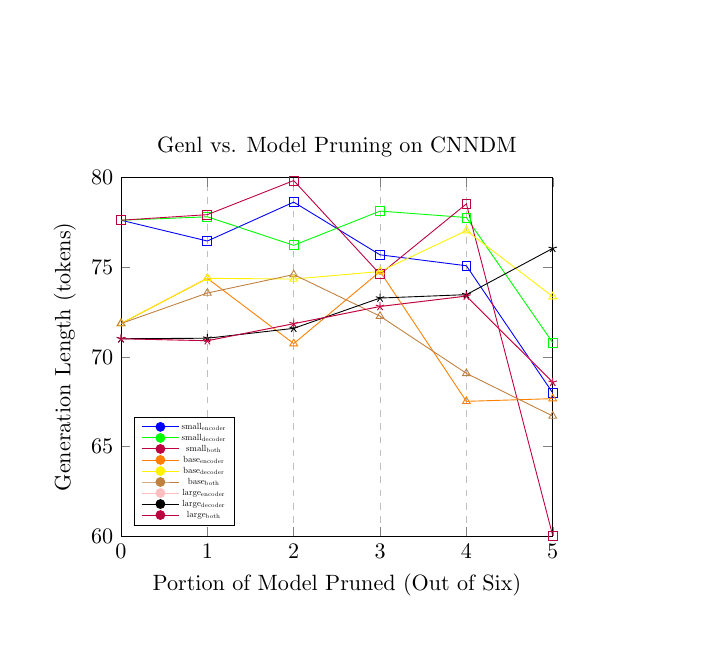
\begin{tikzpicture}
\scalebox{0.8}{
\begin{axis}[
    title={Genl vs. Model Pruning on CNNDM},
    ylabel={Generation Length (tokens)},
    ymin=60, ymax=80,
    ytick={60,65,70,75,80},
    xlabel={Portion of Model Pruned (Out of Six)},
    xmin=0, xmax=5,
    xtick={0,1,2,3,4,5},
    legend pos=south west,
    xmajorgrids=true,
    grid style=dashed,
    legend style={nodes={scale=0.4, transform shape}}, 
    legend image post style={mark=*}
]
\addplot[
    color=blue,
    mark=square,
    ]
    coordinates {
    (0, 77.62) (1, 76.46) (2, 78.63) (3, 75.69) (4, 75.08) (5,67.99)
    };
\addplot[
    color=green,
    mark=square,
    ]
    coordinates {
    (0,  77.62) (1,77.81 ) (2, 76.22) (3, 78.13) (4, 77.77) (5,70.79)
    };  
\addplot[
    color=purple,
    mark=square,
    ]
    coordinates {
    (0,  77.62) (1, 77.93) (2, 79.83 ) (3, 74.61 ) (4, 78.53) (5, 60.03)
    };
\addplot[
    color=orange,
    mark=triangle,
    ]
    coordinates {
    (0,  71.86) (1, 74.38 ) (2, 70.74 ) (3,74.76 ) (4, 67.52 ) (5, 67.67)
    };
\addplot[
    color=yellow,
    mark=triangle,
    ]
    coordinates {
    (0,  71.86) (1,74.38 ) (2, 74.34) (3, 74.76) (4, 77.04) (5, 73.36)
    };  
\addplot[
    color=brown,
    mark=triangle,
    ]
    coordinates {
    (0,  71.86) (1, 73.56 ) (2, 74.59) (3, 72.27) (4, 69.08) (5, 66.70)
    };
\addplot[
    color=pink,
    mark=star,
    ]
    coordinates {
    (0,  71.01) (1, 70.90 ) (2, 71.85 ) (3, 72.81 ) (4, 73.39) (5,68.58)
    };
\addplot[
    color=black,
    mark=star,
    ]
    coordinates {
    (0,  71.01) (1,71.04 ) (2, 71.59) (3, 73.28) (4, 73.47) (5,76.05)
    };  
\addplot[
    color=purple,
    mark=star,
    ]
    coordinates {
    (0,  71.01) (1, 70.9 ) (2, 71.85 ) (3, 72.81 ) (4, 73.39 ) (5, 68.58)
    };
\legend{small\textsubscript{encoder}, small\textsubscript{decoder}, small\textsubscript{both}, base\textsubscript{encoder}, base\textsubscript{decoder}, base\textsubscript{both},large\textsubscript{encoder}, large\textsubscript{decoder}, large\textsubscript{both} }
 \end{axis}}
\end{tikzpicture}
    \caption{Role of scale and compression on generation length}
    \label{fig:scale-genlen1}
\end{figure}
\begin{figure}
    \centering
    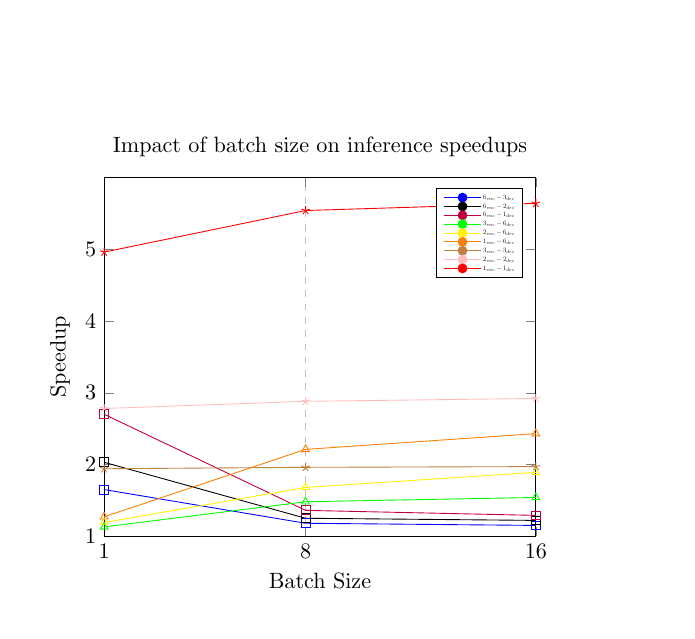
\begin{tikzpicture}
\scalebox{0.8}{
\begin{axis}[
    title={Impact of batch size on inference speedups},
    ylabel={Speedup},
    xlabel={Batch Size},
    ymin=1, ymax=6,
    xmin=1, xmax=16,
    ytick={1,2,3,4,5},
    xtick={1, 8, 16},
    legend pos=north east,
    xmajorgrids=true,
    grid style=dashed,
    legend style={nodes={scale=0.3, transform shape}}, 
    legend image post style={mark=*}
] 
\addplot[
    color=blue,
    mark=square,
    ]
    coordinates {
    (1, 1.65) (8, 1.18) (16,1.15)
    };
\addplot[
    color=black,
    mark=square,
    ]
    coordinates {
    (1, 2.03) (8, 1.25) (16,1.22)
    };
\addplot[
    color=purple,
    mark=square,
    ]
    coordinates {
    (1, 2.70) (8, 1.36) (16,1.29)
    };
\addplot[
    color=green,
    mark=triangle,
    ]
    coordinates {
    (1, 1.13) (8, 1.48) (16,1.54)
    };
\addplot[
    color=yellow,
    mark=triangle,
    ]
    coordinates {
    (1, 1.19) (8, 1.68) (16,1.89)
    };
\addplot[
    color=orange,
    mark=triangle,
    ]
    coordinates {
    (1, 1.27) (8, 2.21) (16,2.43)
    };
\addplot[
    color=brown,
    mark=star,
    ]
    coordinates {
    (1, 1.94) (8, 1.96) (16,1.97)
    }; 
\addplot[
    color=pink,
    mark=star,
    ]
    coordinates {
    (1, 2.78) (8, 2.88) (16,2.92)
    }; 
\addplot[
    color=red,
    mark=star,
    ]
    coordinates {
    (1, 4.96) (8, 5.54) (16,5.64)
    };  
\legend{$6_{enc}-3_{dec}$, $6_{enc}-2_{dec}$,$6_{enc}-1_{dec}$,$3_{enc}-6_{dec}$,$2_{enc}-6_{dec}$,$1_{enc}-6_{dec}$,$3_{enc}-3_{dec}$ ,$2_{enc}-2_{dec}$ ,$1_{enc}-1_{dec}$ }
 \end{axis}}
\end{tikzpicture}
    \caption{Relationship between inference batch size and realized inference speedup with uniform and no uniform pruning of FLAN-T5 large on CNNDM}
    \label{fig:batch-size-scale}
\end{figure}
\subsection{Scale, Pruning and Generated length}
\begin{figure}
    \centering
    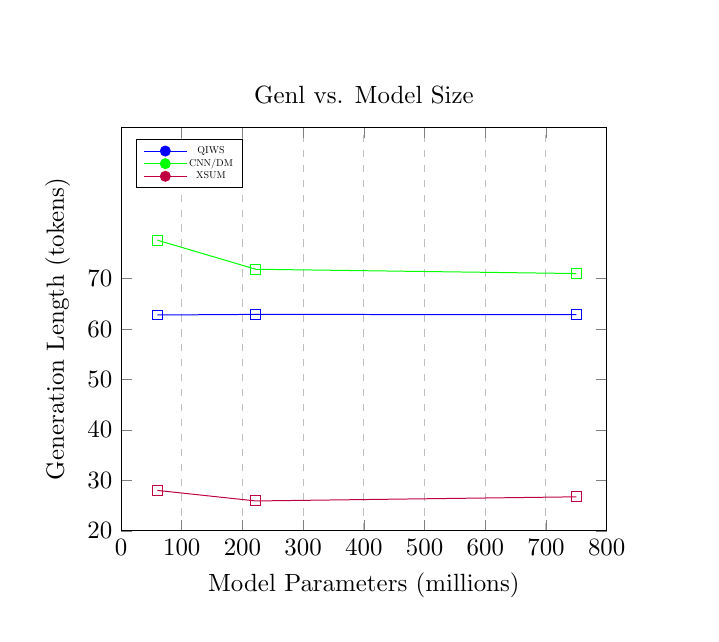
\begin{tikzpicture}
\scalebox{0.9}{
\begin{axis}[
    title={Genl vs. Model Size},
    ylabel={Generation Length (tokens)},
    xlabel={Model Parameters (millions)},
    ymin=20, ymax=100,
    xmin=0, xmax=800,
    ytick={20,30,40,50,60,70},
    xtick={0,100,200,300,400,500,600,700,800},
    legend pos=north west,
    xmajorgrids=true,
    grid style=dashed,
    legend style={nodes={scale=0.4, transform shape}}, 
    legend image post style={mark=*}
]
\addplot[
    color=blue,
    mark=square,
    ]
    coordinates {
    (60,62.79) ( 222,62.91) (750,62.85) 
    };
\addplot[
    color=green,
    mark=square,
    ]
    coordinates {
    (60, 77.62) (222, 71.86) (750,71.01)
    };  
\addplot[
    color=purple,
    mark=square,
    ]
    coordinates {
    (60,28.01) (222, 25.92) (750,26.74)
    };
\legend{QIWS, CNN/DM , XSUM}
 \end{axis}}
\end{tikzpicture}
  \caption{Role of scale on generation length}
    \label{fig:scale-genlen}
\end{figure}
Despite expecting a significant trend in the role of scale and pruning in a generation, we do not see any noticeable trends. As shown in figures \ref{fig:scale-genlen} and \ref{fig:scale-genlen1}, there is no discernible trend of the Role of scale and pruning in generation length. There is a minor jump in generation length from FLAN-T5 small to FLAN-T5 base across all datasets but no such jump from FLAN-T5 base to FLAN-T5 large. We believe this is because the smaller models are less fluent and need more tokens to ensure accurate coverage. As models scale, this is no longer needed, and the models converge to a uniform summary length. 
\subsection{Asymmetry with large batches}
Despite the allures of asymmetrical pruning, it is not without fault. As shown in table \ref{tab:scale-bs-speedup} and figure \ref{fig:batch-size-scale}, the improvements in inference efficiency are heavily influenced by the batch size. When the batch size is minimal, the difference in the type of non-uniformity has a significant impact on inference efficiency. As batches scale, the speedup from encoder only or decoder only becomes much closer and becomes minor when compared to uniform methods. This indicates why further work on improving generative inference methods is highly relevant, as this problem impacts other efficiency-driven processes like CALM \cite{Schuster2022ConfidentAL}.